%% bare_jrnl_transmag.tex
%% V1.4b
%% 2015/08/26
%% by Michael Shell
%% see http://www.michaelshell.org/
%% for current contact information.
%%
%% This is a skeleton file demonstrating the use of IEEEtran.cls
%% (requires IEEEtran.cls version 1.8b or later) with an IEEE 
%% Transactions on Magnetics journal paper.
%%
%% Support sites:
%% http://www.michaelshell.org/tex/ieeetran/
%% http://www.ctan.org/pkg/ieeetran
%% and
%% http://www.ieee.org/

%%*************************************************************************
%% Legal Notice:
%% This code is offered as-is without any warranty either expressed or
%% implied; without even the implied warranty of MERCHANTABILITY or
%% FITNESS FOR A PARTICULAR PURPOSE! 
%% User assumes all risk.
%% In no event shall the IEEE or any contributor to this code be liable for
%% any damages or losses, including, but not limited to, incidental,
%% consequential, or any other damages, resulting from the use or misuse
%% of any information contained here.
%%
%% All comments are the opinions of their respective authors and are not
%% necessarily endorsed by the IEEE.
%%
%% This work is distributed under the LaTeX Project Public License (LPPL)
%% ( http://www.latex-project.org/ ) version 1.3, and may be freely used,
%% distributed and modified. A copy of the LPPL, version 1.3, is included
%% in the base LaTeX documentation of all distributions of LaTeX released
%% 2003/12/01 or later.
%% Retain all contribution notices and credits.
%% ** Modified files should be clearly indicated as such, including  **
%% ** renaming them and changing author support contact information. **
%%*************************************************************************


% *** Authors should verify (and, if needed, correct) their LaTeX system  ***
% *** with the testflow diagnostic prior to trusting their LaTeX platform ***
% *** with production work. The IEEE's font choices and paper sizes can   ***
% *** trigger bugs that do not appear when using other class files.       ***                          ***
% The testflow support page is at:
% http://www.michaelshell.org/tex/testflow/



\documentclass[journal,transmag]{IEEEtran}
%
% If IEEEtran.cls has not been installed into the LaTeX system files,
% manually specify the path to it like:
% \documentclass[journal]{../sty/IEEEtran}





% Some very useful LaTeX packages include:
% (uncomment the ones you want to load)


% *** MISC UTILITY PACKAGES ***
%
%\usepackage{ifpdf}
% Heiko Oberdiek's ifpdf.sty is very useful if you need conditional
% compilation based on whether the output is pdf or dvi.
% usage:
% \ifpdf
%   % pdf code
% \else
%   % dvi code
% \fi
% The latest version of ifpdf.sty can be obtained from:
% http://www.ctan.org/pkg/ifpdf
% Also, note that IEEEtran.cls V1.7 and later provides a builtin
% \ifCLASSINFOpdf conditional that works the same way.
% When switching from latex to pdflatex and vice-versa, the compiler may
% have to be run twice to clear warning/error messages.






% *** CITATION PACKAGES ***
%
%\usepackage{cite}
% cite.sty was written by Donald Arseneau
% V1.6 and later of IEEEtran pre-defines the format of the cite.sty package
% \cite{} output to follow that of the IEEE. Loading the cite package will
% result in citation numbers being automatically sorted and properly
% "compressed/ranged". e.g., [1], [9], [2], [7], [5], [6] without using
% cite.sty will become [1], [2], [5]--[7], [9] using cite.sty. cite.sty's
% \cite will automatically add leading space, if needed. Use cite.sty's
% noadjust option (cite.sty V3.8 and later) if you want to turn this off
% such as if a citation ever needs to be enclosed in parenthesis.
% cite.sty is already installed on most LaTeX systems. Be sure and use
% version 5.0 (2009-03-20) and later if using hyperref.sty.
% The latest version can be obtained at:
% http://www.ctan.org/pkg/cite
% The documentation is contained in the cite.sty file itself.






% *** GRAPHICS RELATED PACKAGES ***
%
\ifCLASSINFOpdf
  % \usepackage[pdftex]{graphicx}
  % declare the path(s) where your graphic files are
  % \graphicspath{{../pdf/}{../jpeg/}}
  % and their extensions so you won't have to specify these with
  % every instance of \includegraphics
  % \DeclareGraphicsExtensions{.pdf,.jpeg,.png}
\else
  % or other class option (dvipsone, dvipdf, if not using dvips). graphicx
  % will default to the driver specified in the system graphics.cfg if no
  % driver is specified.
  % \usepackage[dvips]{graphicx}
  % declare the path(s) where your graphic files are
  % \graphicspath{{../eps/}}
  % and their extensions so you won't have to specify these with
  % every instance of \includegraphics
  % \DeclareGraphicsExtensions{.eps}
\fi
% graphicx was written by David Carlisle and Sebastian Rahtz. It is
% required if you want graphics, photos, etc. graphicx.sty is already
% installed on most LaTeX systems. The latest version and documentation
% can be obtained at: 
% http://www.ctan.org/pkg/graphicx
% Another good source of documentation is "Using Imported Graphics in
% LaTeX2e" by Keith Reckdahl which can be found at:
% http://www.ctan.org/pkg/epslatex
%
% latex, and pdflatex in dvi mode, support graphics in encapsulated
% postscript (.eps) format. pdflatex in pdf mode supports graphics
% in .pdf, .jpeg, .png and .mps (metapost) formats. Users should ensure
% that all non-photo figures use a vector format (.eps, .pdf, .mps) and
% not a bitmapped formats (.jpeg, .png). The IEEE frowns on bitmapped formats
% which can result in "jaggedy"/blurry rendering of lines and letters as
% well as large increases in file sizes.
%
% You can find documentation about the pdfTeX application at:
% http://www.tug.org/applications/pdftex




% *** MATH PACKAGES ***
%
%\usepackage{amsmath}
% A popular package from the American Mathematical Society that provides
% many useful and powerful commands for dealing with mathematics.
%
% Note that the amsmath package sets \interdisplaylinepenalty to 10000
% thus preventing page breaks from occurring within multiline equations. Use:
%\interdisplaylinepenalty=2500
% after loading amsmath to restore such page breaks as IEEEtran.cls normally
% does. amsmath.sty is already installed on most LaTeX systems. The latest
% version and documentation can be obtained at:
% http://www.ctan.org/pkg/amsmath





% *** SPECIALIZED LIST PACKAGES ***
%
%\usepackage{algorithmic}
% algorithmic.sty was written by Peter Williams and Rogerio Brito.
% This package provides an algorithmic environment fo describing algorithms.
% You can use the algorithmic environment in-text or within a figure
% environment to provide for a floating algorithm. Do NOT use the algorithm
% floating environment provided by algorithm.sty (by the same authors) or
% algorithm2e.sty (by Christophe Fiorio) as the IEEE does not use dedicated
% algorithm float types and packages that provide these will not provide
% correct IEEE style captions. The latest version and documentation of
% algorithmic.sty can be obtained at:
% http://www.ctan.org/pkg/algorithms
% Also of interest may be the (relatively newer and more customizable)
% algorithmicx.sty package by Szasz Janos:
% http://www.ctan.org/pkg/algorithmicx




% *** ALIGNMENT PACKAGES ***
%
%\usepackage{array}
% Frank Mittelbach's and David Carlisle's array.sty patches and improves
% the standard LaTeX2e array and tabular environments to provide better
% appearance and additional user controls. As the default LaTeX2e table
% generation code is lacking to the point of almost being broken with
% respect to the quality of the end results, all users are strongly
% advised to use an enhanced (at the very least that provided by array.sty)
% set of table tools. array.sty is already installed on most systems. The
% latest version and documentation can be obtained at:
% http://www.ctan.org/pkg/array


% IEEEtran contains the IEEEeqnarray family of commands that can be used to
% generate multiline equations as well as matrices, tables, etc., of high
% quality.




% *** SUBFIGURE PACKAGES ***
%\ifCLASSOPTIONcompsoc
%  \usepackage[caption=false,font=normalsize,labelfont=sf,textfont=sf]{subfig}
%\else
%  \usepackage[caption=false,font=footnotesize]{subfig}
%\fi
% subfig.sty, written by Steven Douglas Cochran, is the modern replacement
% for subfigure.sty, the latter of which is no longer maintained and is
% incompatible with some LaTeX packages including fixltx2e. However,
% subfig.sty requires and automatically loads Axel Sommerfeldt's caption.sty
% which will override IEEEtran.cls' handling of captions and this will result
% in non-IEEE style figure/table captions. To prevent this problem, be sure
% and invoke subfig.sty's "caption=false" package option (available since
% subfig.sty version 1.3, 2005/06/28) as this is will preserve IEEEtran.cls
% handling of captions.
% Note that the Computer Society format requires a larger sans serif font
% than the serif footnote size font used in traditional IEEE formatting
% and thus the need to invoke different subfig.sty package options depending
% on whether compsoc mode has been enabled.
%
% The latest version and documentation of subfig.sty can be obtained at:
% http://www.ctan.org/pkg/subfig



% *** FLOAT PACKAGES ***
%
%\usepackage{fixltx2e}
% fixltx2e, the successor to the earlier fix2col.sty, was written by
% Frank Mittelbach and David Carlisle. This package corrects a few problems
% in the LaTeX2e kernel, the most notable of which is that in current
% LaTeX2e releases, the ordering of single and double column floats is not
% guaranteed to be preserved. Thus, an unpatched LaTeX2e can allow a
% single column figure to be placed prior to an earlier double column
% figure.
% Be aware that LaTeX2e kernels dated 2015 and later have fixltx2e.sty's
% corrections already built into the system in which case a warning will
% be issued if an attempt is made to load fixltx2e.sty as it is no longer
% needed.
% The latest version and documentation can be found at:
% http://www.ctan.org/pkg/fixltx2e


%\usepackage{stfloats}
% stfloats.sty was written by Sigitas Tolusis. This package gives LaTeX2e
% the ability to do double column floats at the bottom of the page as well
% as the top. (e.g., "\begin{figure*}[!b]" is not normally possible in
% LaTeX2e). It also provides a command:
%\fnbelowfloat
% to enable the placement of footnotes below bottom floats (the standard
% LaTeX2e kernel puts them above bottom floats). This is an invasive package
% which rewrites many portions of the LaTeX2e float routines. It may not work
% with other packages that modify the LaTeX2e float routines. The latest
% version and documentation can be obtained at:
% http://www.ctan.org/pkg/stfloats
% Do not use the stfloats baselinefloat ability as the IEEE does not allow
% \baselineskip to stretch. Authors submitting work to the IEEE should note
% that the IEEE rarely uses double column equations and that authors should try
% to avoid such use. Do not be tempted to use the cuted.sty or midfloat.sty
% packages (also by Sigitas Tolusis) as the IEEE does not format its papers in
% such ways.
% Do not attempt to use stfloats with fixltx2e as they are incompatible.
% Instead, use Morten Hogholm'a dblfloatfix which combines the features
% of both fixltx2e and stfloats:
%
% \usepackage{dblfloatfix}
% The latest version can be found at:
% http://www.ctan.org/pkg/dblfloatfix




%\ifCLASSOPTIONcaptionsoff
%  \usepackage[nomarkers]{endfloat}
% \let\MYoriglatexcaption\caption
% \renewcommand{\caption}[2][\relax]{\MYoriglatexcaption[#2]{#2}}
%\fi
% endfloat.sty was written by James Darrell McCauley, Jeff Goldberg and 
% Axel Sommerfeldt. This package may be useful when used in conjunction with 
% IEEEtran.cls'  captionsoff option. Some IEEE journals/societies require that
% submissions have lists of figures/tables at the end of the paper and that
% figures/tables without any captions are placed on a page by themselves at
% the end of the document. If needed, the draftcls IEEEtran class option or
% \CLASSINPUTbaselinestretch interface can be used to increase the line
% spacing as well. Be sure and use the nomarkers option of endfloat to
% prevent endfloat from "marking" where the figures would have been placed
% in the text. The two hack lines of code above are a slight modification of
% that suggested by in the endfloat docs (section 8.4.1) to ensure that
% the full captions always appear in the list of figures/tables - even if
% the user used the short optional argument of \caption[]{}.
% IEEE papers do not typically make use of \caption[]'s optional argument,
% so this should not be an issue. A similar trick can be used to disable
% captions of packages such as subfig.sty that lack options to turn off
% the subcaptions:
% For subfig.sty:
% \let\MYorigsubfloat\subfloat
% \renewcommand{\subfloat}[2][\relax]{\MYorigsubfloat[]{#2}}
% However, the above trick will not work if both optional arguments of
% the \subfloat command are used. Furthermore, there needs to be a
% description of each subfigure *somewhere* and endfloat does not add
% subfigure captions to its list of figures. Thus, the best approach is to
% avoid the use of subfigure captions (many IEEE journals avoid them anyway)
% and instead reference/explain all the subfigures within the main caption.
% The latest version of endfloat.sty and its documentation can obtained at:
% http://www.ctan.org/pkg/endfloat
%
% The IEEEtran \ifCLASSOPTIONcaptionsoff conditional can also be used
% later in the document, say, to conditionally put the References on a 
% page by themselves.




% *** PDF, URL AND HYPERLINK PACKAGES ***
%
%\usepackage{url}
% url.sty was written by Donald Arseneau. It provides better support for
% handling and breaking URLs. url.sty is already installed on most LaTeX
% systems. The latest version and documentation can be obtained at:
% http://www.ctan.org/pkg/url
% Basically, \url{my_url_here}.




% *** Do not adjust lengths that control margins, column widths, etc. ***
% *** Do not use packages that alter fonts (such as pslatex).         ***
% There should be no need to do such things with IEEEtran.cls V1.6 and later.
% (Unless specifically asked to do so by the journal or conference you plan
% to submit to, of course. )

\usepackage{amsmath}
\usepackage{subcaption}
\usepackage{graphicx}
\usepackage{url}
\usepackage{array}
\begin{document}
%
% paper title
% Titles are generally capitalized except for words such as a, an, and, as,
% at, but, by, for, in, nor, of, on, or, the, to and up, which are usually
% not capitalized unless they are the first or last word of the title.
% Linebreaks \\ can be used within to get better formatting as desired.
% Do not put math or special symbols in the title.
\title{SmartCam Module \\ Innovating Self-Learning Software for Intelligent Vision}



% author names and affiliations
% transmag papers use the long conference author name format.

\author{\IEEEauthorblockN{SangWoo Park\IEEEauthorrefmark{1},
Hantao Fu\IEEEauthorrefmark{1},
~\IEEEmembership{ELEC 594, Capstone Project}}
\IEEEauthorblockA{\IEEEauthorrefmark{1}Master's of Electrical \& Computer Engineering, Rice University, Houston, TX 77005 USA}

\thanks{Manuscript revised March 24, 2025. Corresponding author: SangWoo P.}}



% The paper headers
\markboth{MECE ELEC 594 Report of IEEE \LaTeX\ March~2025}%
{Shell \MakeLowercase{\textit{et al.}}: SmartCam Module}
% The only time the second header will appear is for the odd numbered pages
% after the title page when using the twoside option.
% 
% *** Note that you probably will NOT want to include the author's ***
% *** name in the headers of peer review papers.                   ***
% You can use \ifCLASSOPTIONpeerreview for conditional compilation here if
% you desire.




% If you want to put a publisher's ID mark on the page you can do it like
% this:
%\IEEEpubid{0000--0000/00\$00.00~\copyright~2015 IEEE}
% Remember, if you use this you must call \IEEEpubidadjcol in the second
% column for its text to clear the IEEEpubid mark.



% use for special paper notices
%\IEEEspecialpapernotice{(Invited Paper)}


% for Transactions on Magnetics papers, we must declare the abstract and
% index terms PRIOR to the title within the \IEEEtitleabstractindextext
% IEEEtran command as these need to go into the title area created by
% \maketitle.
% As a general rule, do not put math, special symbols or citations
% in the abstract or keywords.
\IEEEtitleabstractindextext{%
\begin{abstract}
In this project, KTM Technology aims to expand into the professional camera module sector by developing an integrated training module that combines hardware and software to optimize costs. To achieve this, we plan to develop a training software for camera modules capable of learning from real-world data under various conditions.Through our initial research, we have identified seven key solutions that provide valuable insights into industry approaches [1]–[7]. Inspired by these references, we will further explore and refine more frameworks to guide our development. Our proposed solution will build on existing methodologies across various fields, including drones, medical devices, and material characterization equipment, while incorporating enhanced features to improve performance and versatility.The primary goal for this semester is to implement our training software into commercially available camera hardware, enabling it to identify specific objects with reasonable accuracy. Our focus will be on establishing a robust framework for the camera module, while aspects such as stability, error minimization, and seamless functionality will be addressed in the following semester.
\end{abstract}

% Note that keywords are not normally used for peerreview papers.
\begin{IEEEkeywords}
Camera Vision, AI, Training module, Big data, Machine learning, ADAS, Autonomous driving, Automotive.
\end{IEEEkeywords}}



% make the title area
\maketitle


% To allow for easy dual compilation without having to reenter the
% abstract/keywords data, the \IEEEtitleabstractindextext text will
% not be used in maketitle, but will appear (i.e., to be "transported")
% here as \IEEEdisplaynontitleabstractindextext when the compsoc 
% or transmag modes are not selected <OR> if conference mode is selected 
% - because all conference papers position the abstract like regular
% papers do.
\IEEEdisplaynontitleabstractindextext
% \IEEEdisplaynontitleabstractindextext has no effect when using
% compsoc or transmag under a non-conference mode.







% For peer review papers, you can put extra information on the cover
% page as needed:
% \ifCLASSOPTIONpeerreview
% \begin{center} \bfseries EDICS Category: 3-BBND \end{center}
% \fi
%
% For peerreview papers, this IEEEtran command inserts a page break and
% creates the second title. It will be ignored for other modes.
%\IEEEpeerreviewmaketitle



\section{Introduction}
% The very first letter is a 2 line initial drop letter followed
% by the rest of the first word in caps.
% 
% form to use if the first word consists of a single letter:
% \IEEEPARstart{A}{demo} file is ....
% 
% form to use if you need the single drop letter followed by
% normal text (unknown if ever used by the IEEE):
% \IEEEPARstart{A}{}demo file is ....
% 
% Some journals put the first two words in caps:
% \IEEEPARstart{T}{his demo} file is ....
% 
% Here we have the typical use of a "T" for an initial drop letter
% and "HIS" in caps to complete the first word.


%\subsection{Background \& Industry Relevance}
\IEEEPARstart
The rapid advancement of electric vehicles has intensified the demand for high-performance vision systems capable of real-time environmental perception and decision-making. As automotive manufacturers integrate sophisticated driver-assistance and autonomous navigation technologies, intelligent camera modules must evolve beyond static recognition models to incorporate dynamic learning capabilities. Conventional vision systems, constrained by predefined datasets and manual calibration, struggle to adapt to complex driving environments. This project aims to develop a next-generation AI-powered smart camera module that autonomously refines its object detection and classification algorithms, optimizing performance across diverse operational conditions. By leveraging cutting-edge machine learning methodologies, the proposed system aspires to bridge the gap between traditional camera modules and fully autonomous perception frameworks.
% You must have at least 2 lines in the paragraph with the drop letter
% (should never be an issue)


\subsection{Goal \& Motivation}

This project seeks to develop an advanced AI-driven training module for camera systems, drawing inspiration from Tesla’s Full Self-Driving (FSD) architecture\cite{FSD}\cite{Autopilot}, whose features are shown in Table~\ref{tab:FSD_Feature}. The proposed system will employ deep learning techniques to enable real-time adaptability, improving object recognition accuracy under dynamic conditions. The envisioned technology holds significant potential for integration into Hyundai Motors' next-generation autonomous vehicle platforms.

\begin{table*}[t]
\centering
\caption{FSD Main Features}
\label{tab:FSD_Feature}
\begin{tabular}{|c|p{12cm}|}  
\hline
\textbf{Feature} & \multicolumn{1}{c|}{\textbf{Mechanism}} \\
\hline
Traffic Light Detection & Uses cameras and deep neural networks (DNNs) to recognize red, yellow, and green lights. \\
\hline
Speed Limit Sign Recognition & Reads speed limit signs via vision-based object detection and cross-references with GPS and map data. \\
\hline
Stop Sign and Yield Sign Detection & Identifies standard stop and yield signs through camera-based object recognition. \\
\hline
Decision Making & FSD slows down and stops for detected traffic signals or stop signs, requiring driver input for confirmation. \\
\hline
Occlusion Handling & Uses context-aware AI to infer missing or obscured signs based on surrounding traffic behavior. \\
\hline
Nighttime and Low Visibility Performance & Uses enhanced image processing and exposure control for nighttime detection. \\
\hline
Continuous Learning and Updates & Improves detection with over-the-air (OTA) software updates and data from Tesla’s fleet. \\
\hline
\end{tabular}
\end{table*}




Current market solutions exhibit limitations in scalability, adaptability, and computational efficiency. Many commercially available camera modules lack the capability to autonomously train on domain-specific datasets, restricting their applicability in automotive, medical, and industrial settings. Furthermore, proprietary AI training software presents cost barriers that hinder widespread adoption. By developing an intelligent, self-learning training framework, this project aims to establish a competitive edge by enhancing operational flexibility, reducing dependency on predefined datasets, and improving cost efficiency. The resulting system is expected to contribute to the advancement of adaptive vision technologies within the broader autonomous systems landscape.

% needed in second column of first page if using \IEEEpubid
%\IEEEpubidadjcol

\subsection{Related Work}

Significant research has been conducted in AI-driven vision training and object recognition. Kumar et al. \cite{SelfDriving} demonstrated the feasibility of cost-efficient self-driving navigation using neural networks and computer vision, while Ismael et al. \cite{Controlling Mobile Robot} explored OCR-based mobile robot navigation. Brady \cite{Smart Cameras} examined architectural advancements in smart camera systems, emphasizing real-time computational efficiency, whereas Hong \cite{Design and Realization} investigated AI-driven fire detection for hazard mitigation. Open-source projects such as Camera-trap-classifier \cite{Camera-trap-classifier}, UniScene \cite{UniScene}, and Autodrone \cite{Autodrone} have contributed practical implementations of AI-based vision training methodologies.

Building on these studies, this project will advance AI-driven camera module capabilities by integrating adaptive training frameworks that enhance recognition performance, computational efficiency, and real-world deployability. This approach seeks to position the developed technology as a viable solution within the competitive landscape of intelligent automotive vision systems



%{T}{his} demo file is intended to serve as a ``starter file''
%for IEEE \textsc{Transactions on Magnetics} journal papers produced under %\LaTeX\ using
%IEEEtran.cls version 1.8b and later.
% You must have at least 2 lines in the paragraph with the drop letter
% (should never be an issue)

% An example of a floating figure using the graphicx package.
% Note that \label must occur AFTER (or within) \caption.
% For figures, \caption should occur after the \includegraphics.
% Note that IEEEtran v1.7 and later has special internal code that
% is designed to preserve the operation of \label within \caption
% even when the captionsoff option is in effect. However, because
% of issues like this, it may be the safest practice to put all your
% \label just after \caption rather than within \caption{}.
%
% Reminder: the "draftcls" or "draftclsnofoot", not "draft", class
% option should be used if it is desired that the figures are to be
% displayed while in draft mode.
%
%\begin{figure}[!t]
%\centering
%\includegraphics[width=2.5in]{myfigure}
% where an .eps filename suffix will be assumed under latex, 
% and a .pdf suffix will be assumed for pdflatex; or what has been declared
% via \DeclareGraphicsExtensions.
%\caption{Simulation results for the network.}
%\label{fig_sim}
%\end{figure}

% Note that the IEEE typically puts floats only at the top, even when this
% results in a large percentage of a column being occupied by floats.


% An example of a double column floating figure using two subfigures.
% (The subfig.sty package must be loaded for this to work.)
% The subfigure \label commands are set within each subfloat command,
% and the \label for the overall figure must come after \caption.
% \hfil is used as a separator to get equal spacing.
% Watch out that the combined width of all the subfigures on a 
% line do not exceed the text width or a line break will occur.
%
%\begin{figure*}[!t]
%\centering
%\subfloat[Case I]{\includegraphics[width=2.5in]{box}%
%\label{fig_first_case}}
%\hfil
%\subfloat[Case II]{\includegraphics[width=2.5in]{box}%
%\label{fig_second_case}}
%\caption{Simulation results for the network.}
%\label{fig_sim}
%\end{figure*}
%
% Note that often IEEE papers with subfigures do not employ subfigure
% captions (using the optional argument to \subfloat[]), but instead will
% reference/describe all of them (a), (b), etc., within the main caption.
% Be aware that for subfig.sty to generate the (a), (b), etc., subfigure
% labels, the optional argument to \subfloat must be present. If a
% subcaption is not desired, just leave its contents blank,
% e.g., \subfloat[].


% An example of a floating table. Note that, for IEEE style tables, the
% \caption command should come BEFORE the table and, given that table
% captions serve much like titles, are usually capitalized except for words
% such as a, an, and, as, at, but, by, for, in, nor, of, on, or, the, to
% and up, which are usually not capitalized unless they are the first or
% last word of the caption. Table text will default to \footnotesize as
% the IEEE normally uses this smaller font for tables.
% The \label must come after \caption as always.
%
%\begin{table}[!t]
%% increase table row spacing, adjust to taste
%\renewcommand{\arraystretch}{1.3}
% if using array.sty, it might be a good idea to tweak the value of
% \extrarowheight as needed to properly center the text within the cells
%\caption{An Example of a Table}
%\label{table_example}
%\centering
%% Some packages, such as MDW tools, offer better commands for making tables
%% than the plain LaTeX2e tabular which is used here.
%\begin{tabular}{|c||c|}
%\hline
%One & Two\\
%\hline
%Three & Four\\
%\hline
%\end{tabular}
%\end{table}


% Note that the IEEE does not put floats in the very first column
% - or typically anywhere on the first page for that matter. Also,
% in-text middle ("here") positioning is typically not used, but it
% is allowed and encouraged for Computer Society conferences (but
% not Computer Society journals). Most IEEE journals/conferences use
% top floats exclusively. 
% Note that, LaTeX2e, unlike IEEE journals/conferences, places
% footnotes above bottom floats. This can be corrected via the
% \fnbelowfloat command of the stfloats package.
\vspace{0.05cm}
\section{Methodology}

%\subsection{System Framework}

In this project, we aim to develop an object recognition software for the in-vehicle camera module of autonomous vehicles, designed to help the car identify common objects on the road. Our objective is to ensure the software incorporates the following four key features, as shown in Figure~\ref{fig:feature}: 

\begin{figure}[h]
    \centering
    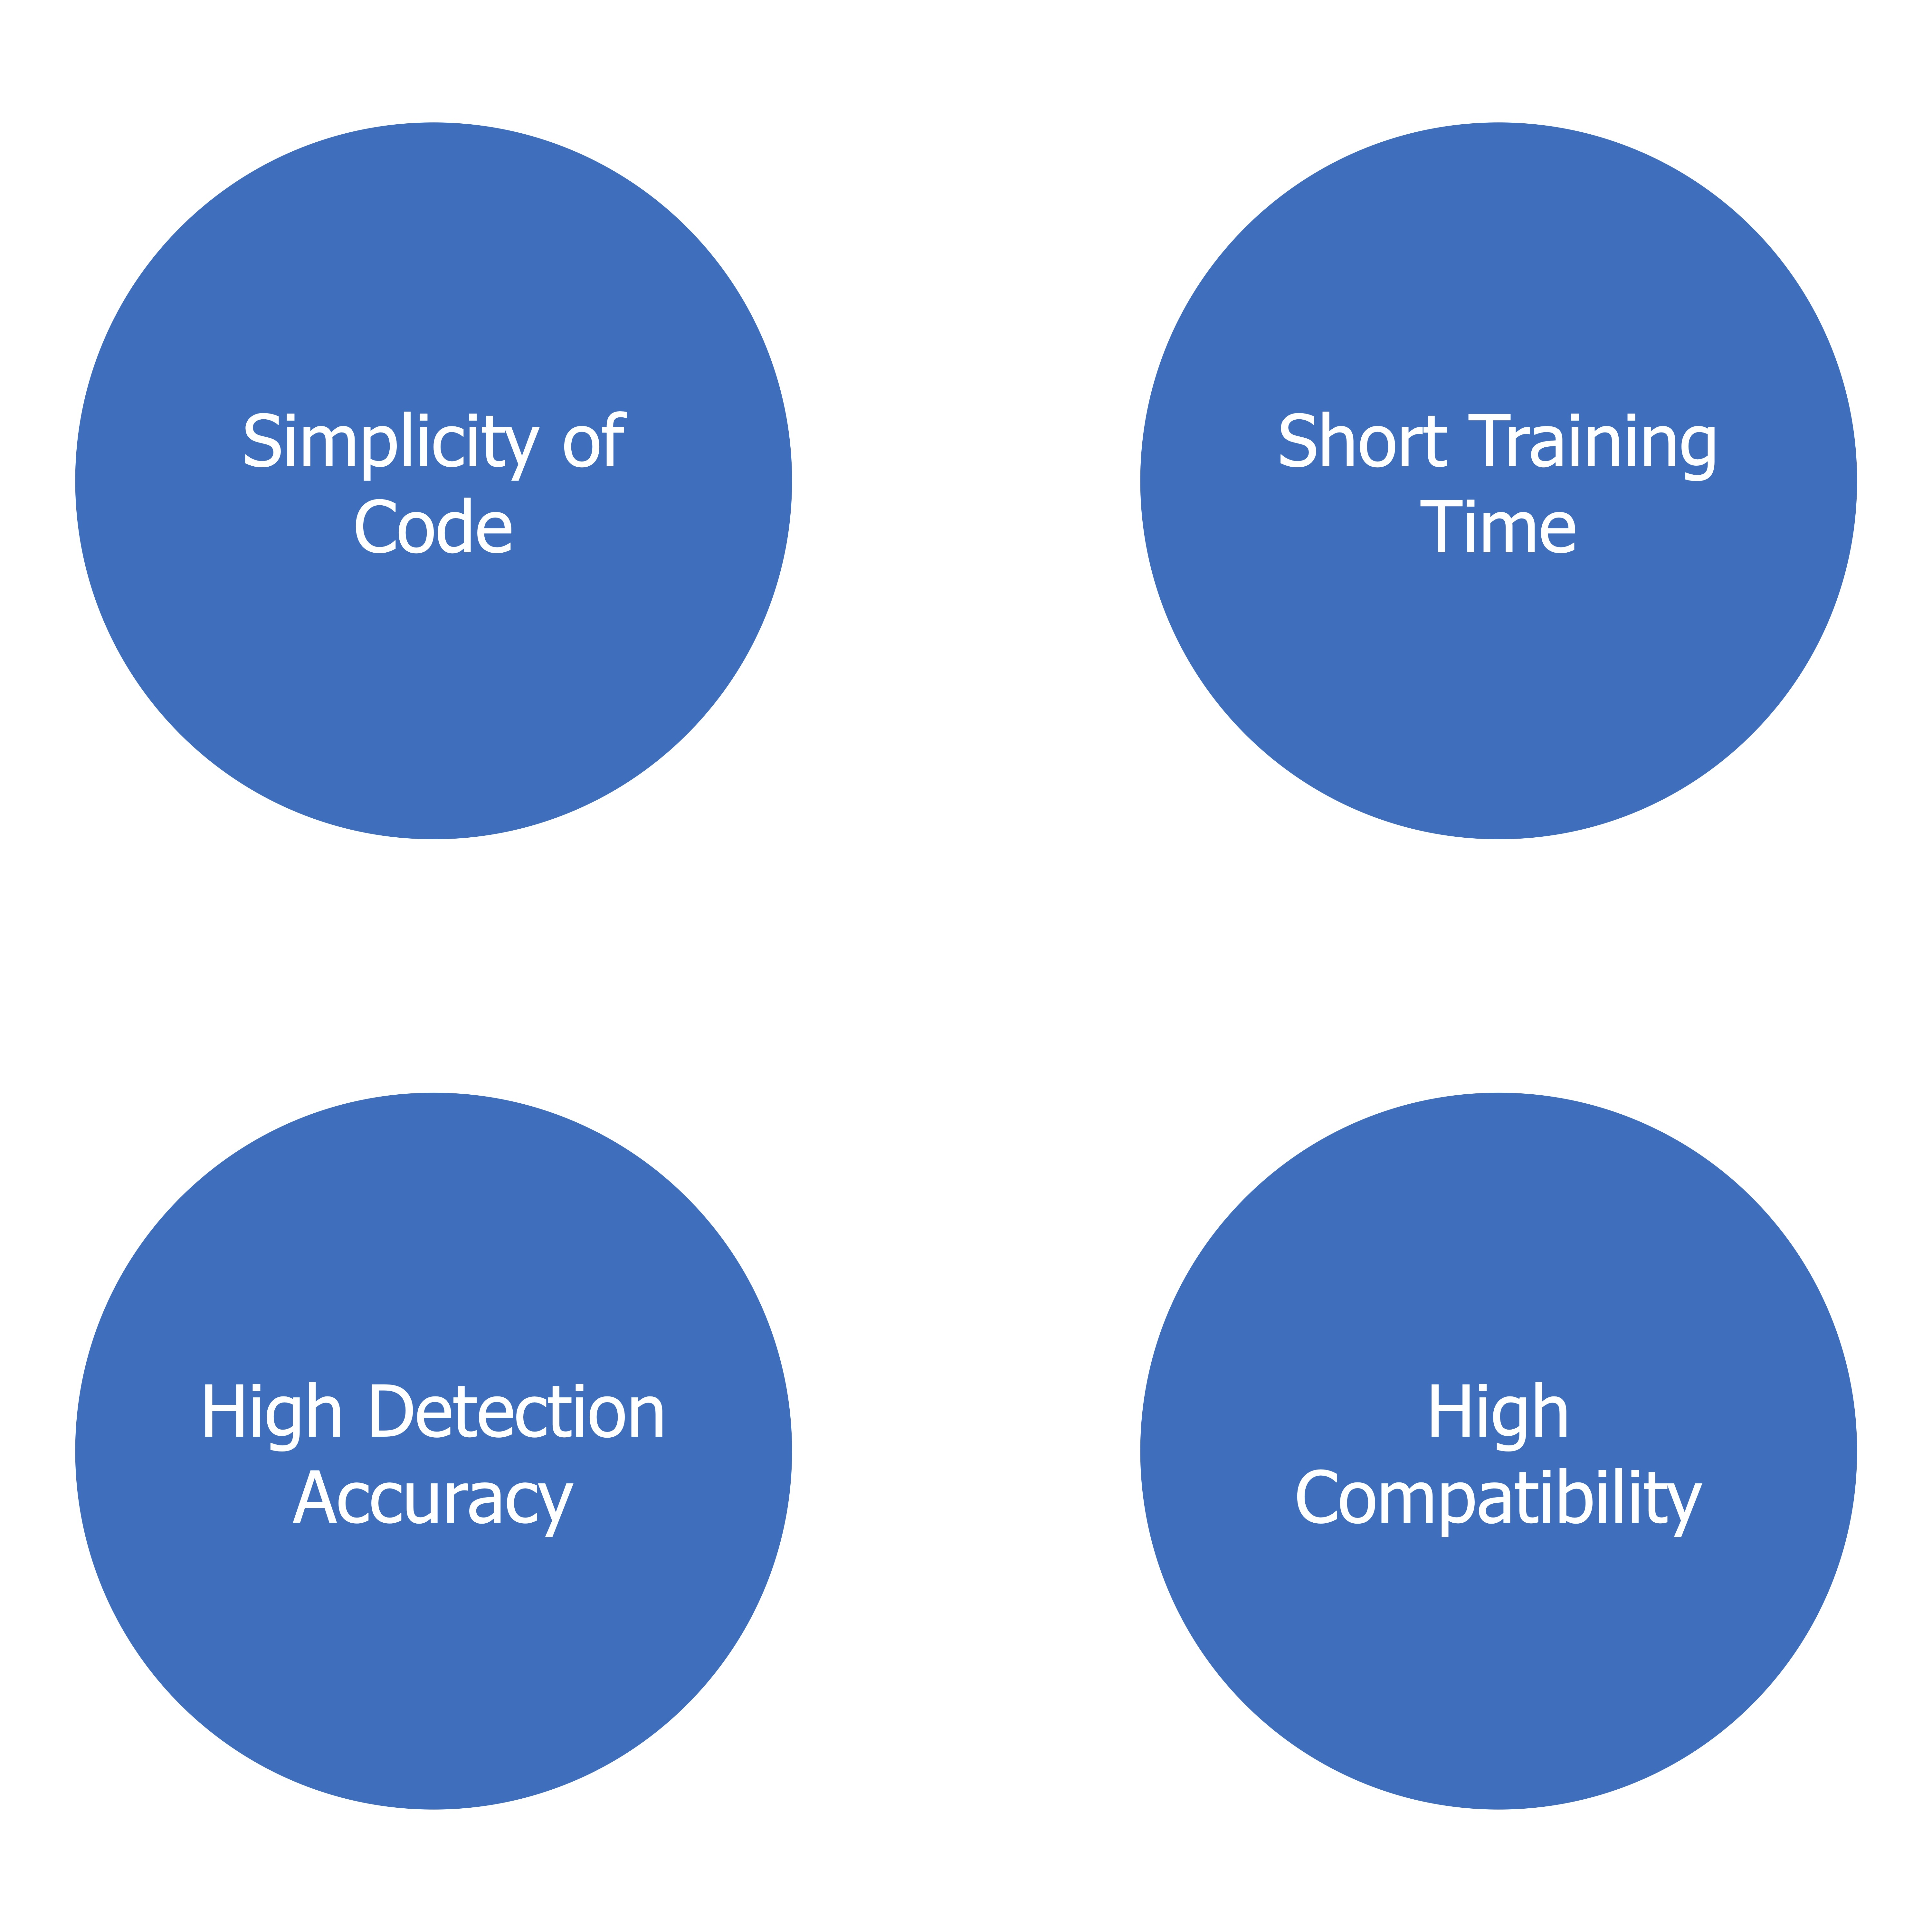
\includegraphics[width=0.25\textwidth]{Feature.jpg} 
    \caption{4 Key Features of our Solution}
    \label{fig:feature}
\end{figure}

\vspace{0.1cm}
i. \textbf{Simplicity of Code} A concise piece of code has greater scalability, allowing us to develop as many features as possible while consuming as little time as possible.

ii. \textbf{Short Training Time} Consuming less time during the training process ensures that the camera module can train on more data within a given time unit, using a larger dataset to pursue higher performance.

iii. \textbf{High Detection Accuracy} Most modules only detect the objects in rectangular shape, but we are expecting detecting its border preciser to enhance accuracy and fast response. 

iv. \textbf{High Compatibility} It has to be user-friendly, so module could be compatible with all camera modules regardless of its generation.

To simplify a complex problem, our approach is divided into three main components, as shown in Figure~\ref{fig:method}. Each part is addressed sequentially, allowing for focused development and easier troubleshooting. Once all components are completed, they will be integrated into a unified system to form the final deliverable of our project. 

\begin{figure}[h]
    \centering
    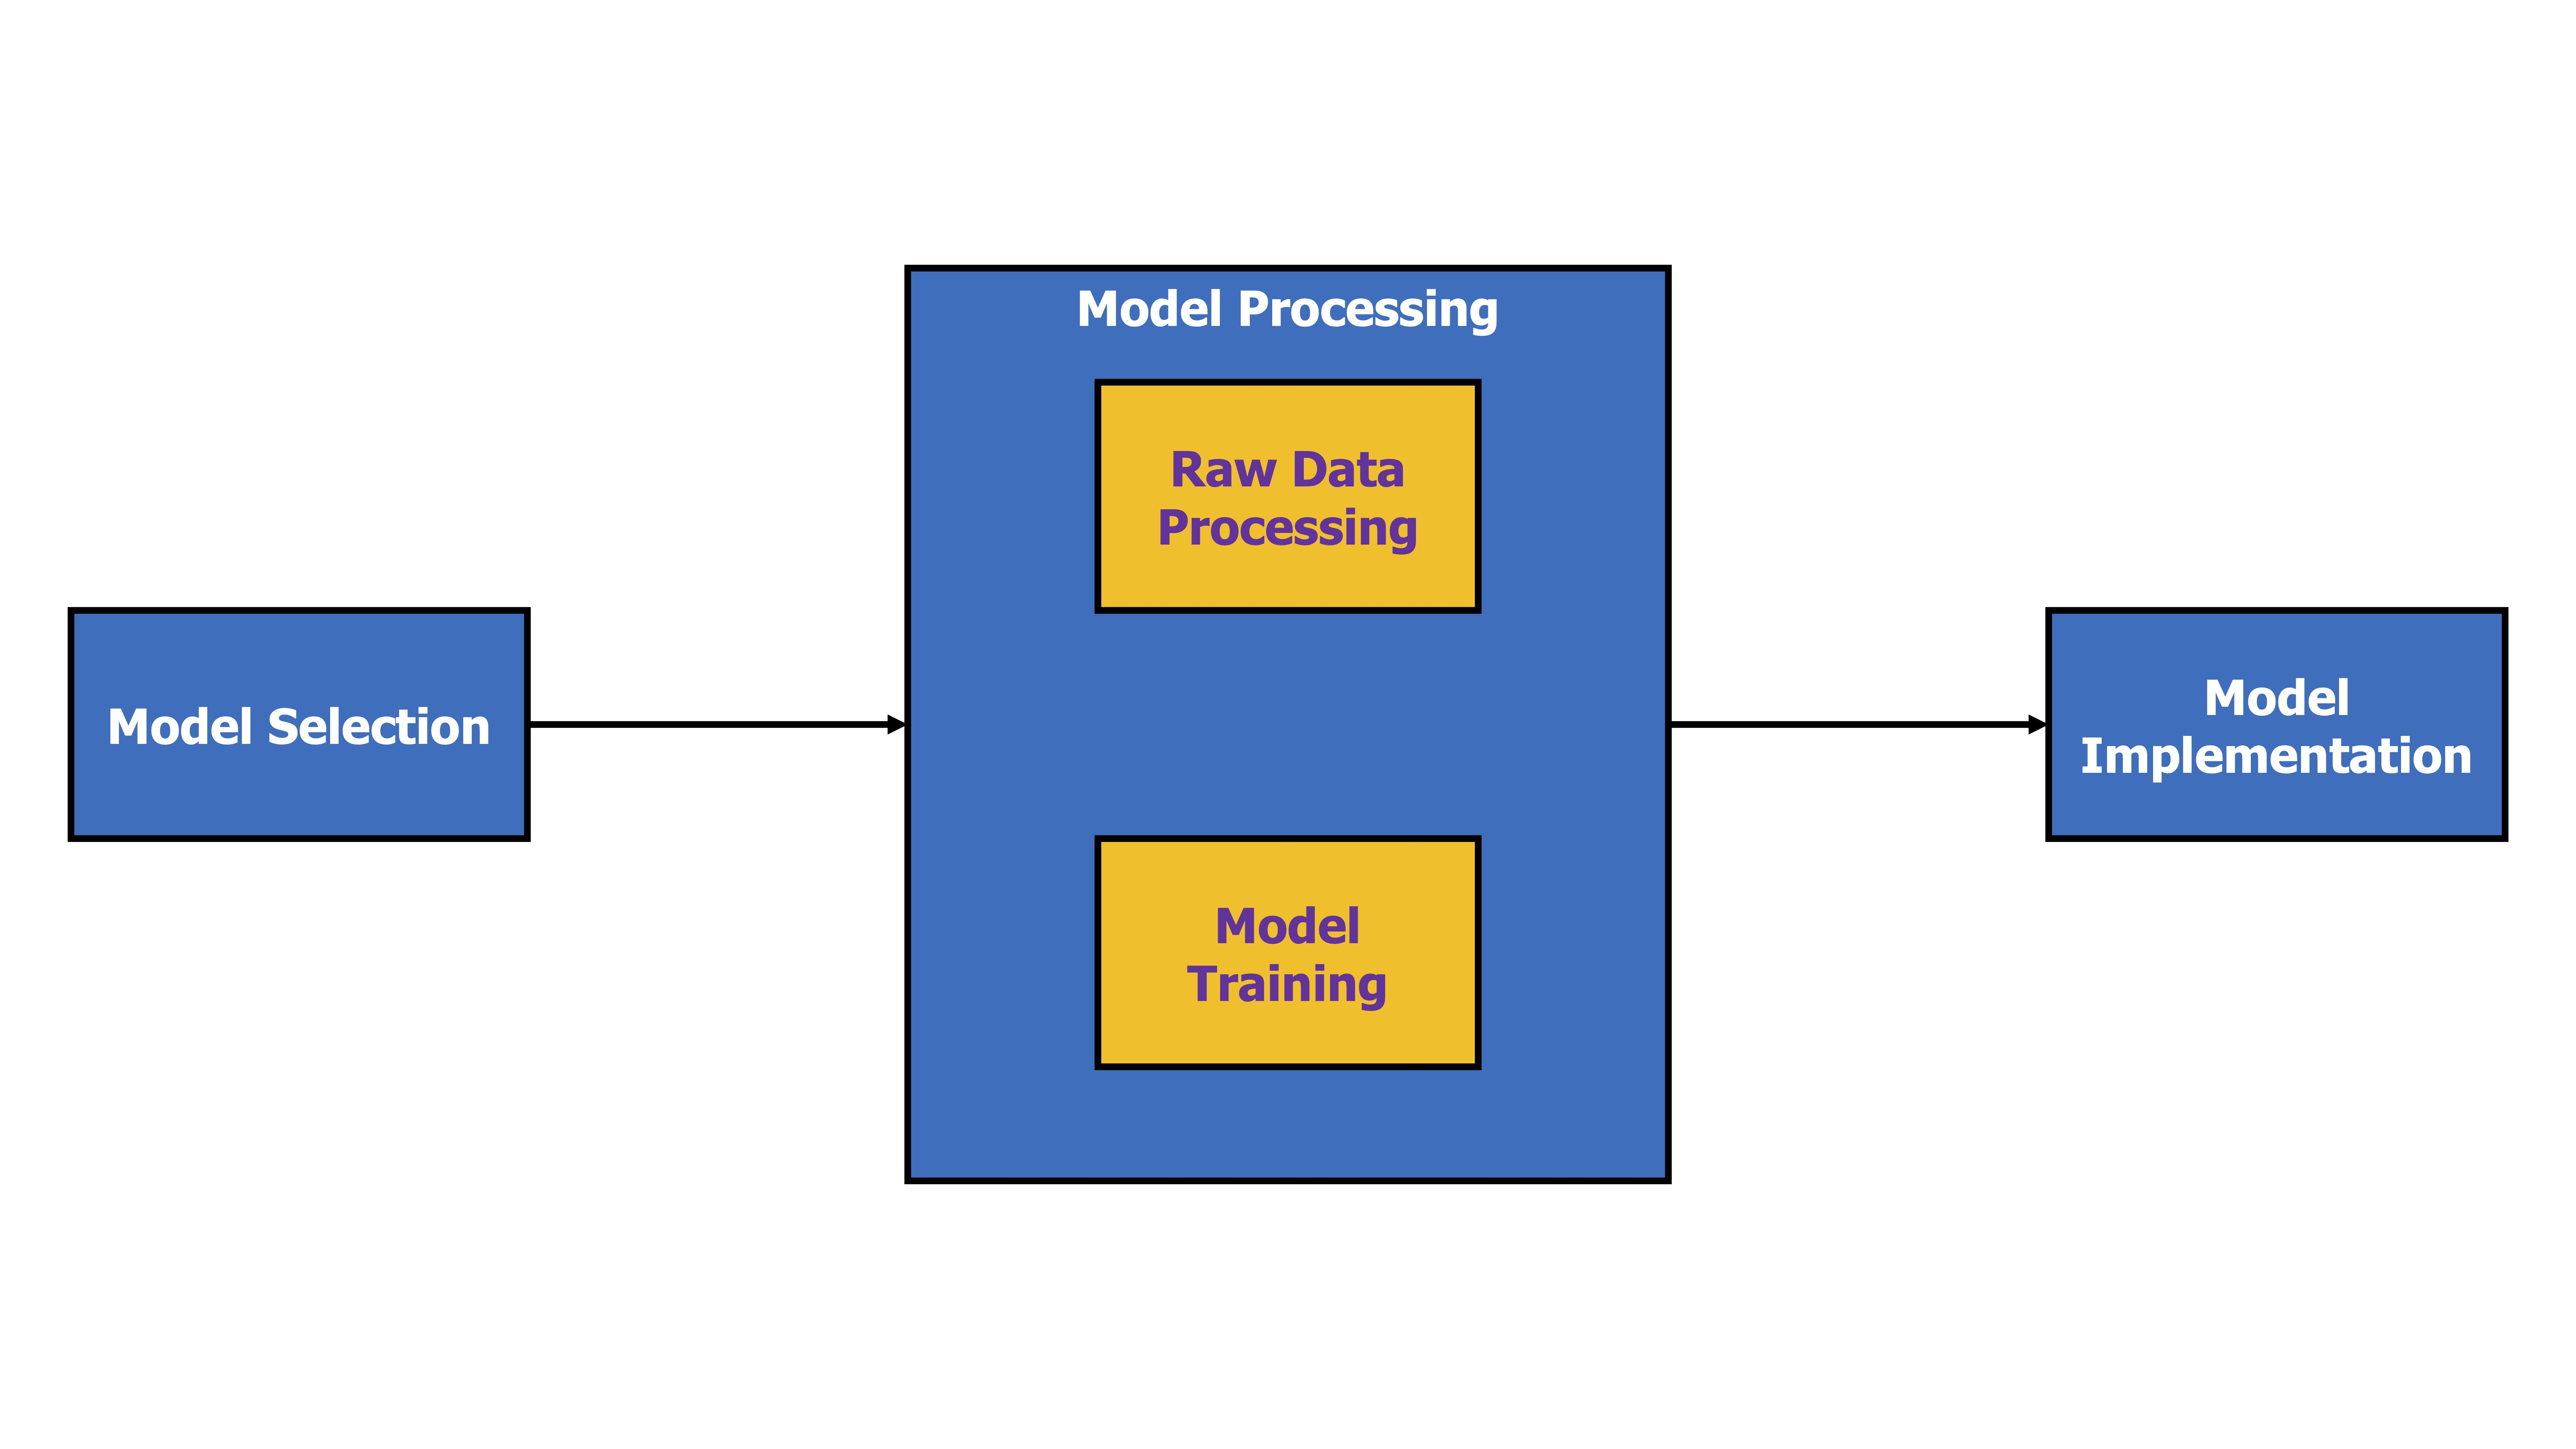
\includegraphics[width=0.45\textwidth]{Methods.jpg} 
    \caption{The Method of this Project}
    \label{fig:method}
\end{figure}

\subsection{Deep Learning Model Selection \& Optimization}


This project employs the You Only Look Once (\textbf{YOLO}) algorithm to enhance the object detection capabilities of a camera system. YOLO is a state-of-the-art deep learning model known for its real-time speed, high accuracy, and computational efficiency. Unlike two-stage detectors like Faster R-CNN, YOLO follows a single-stage framework, processing an entire image in one forward pass to perform classification and localization simultaneously. This eliminates the need for region proposals, significantly reducing computational overhead. Figure~\ref{fig:external_yolo} shows how it works[8]: 

i. \textbf{Image Preprocessing} The input image is resized to a fixed dimension (e.g., 416 × 416 or 608 × 608) and normalized to enhance computational efficiency. The resized image is then passed through a CNN backbone for feature extraction.


ii. \textbf{Grid-Based Localization} The image is divided into an $S \times S$ grid, where each grid cell is responsible for detecting objects whose centers fall within it. Each cell predicts multiple bounding boxes, along with confidence scores and class probabilities.

iii. \textbf{Bounding Box Prediction} Each grid cell predicts $B$ bounding boxes, where each bounding box consists of:
\begin{itemize}
  \setlength{\itemindent}{1em} 
  \item $(x, y)$: The center coordinates relative to the grid cell.
  \item $(w, h)$: The width and height normalized to the entire image.
  \item Confidence score: The likelihood that the bounding box contains an object.
  \item Class probabilities: The probability distribution over predefined object categories.
\end{itemize}

iv. \textbf{Non-Maximum Suppression} To eliminate redundant bounding boxes, YOLO employs Non-Maximum Suppression \textbf{(NMS)}, which:
\begin{itemize}
  \setlength{\itemindent}{2em} 
  \item Selects the bounding box with the highest confidence score.
  \item Removes overlapping boxes with an Intersection over Union \textbf{(IoU)} threshold (e.g., 0.5).
  \item Retains only the most relevant bounding boxes.
\end{itemize}

\begin{figure}[h]
    \centering
    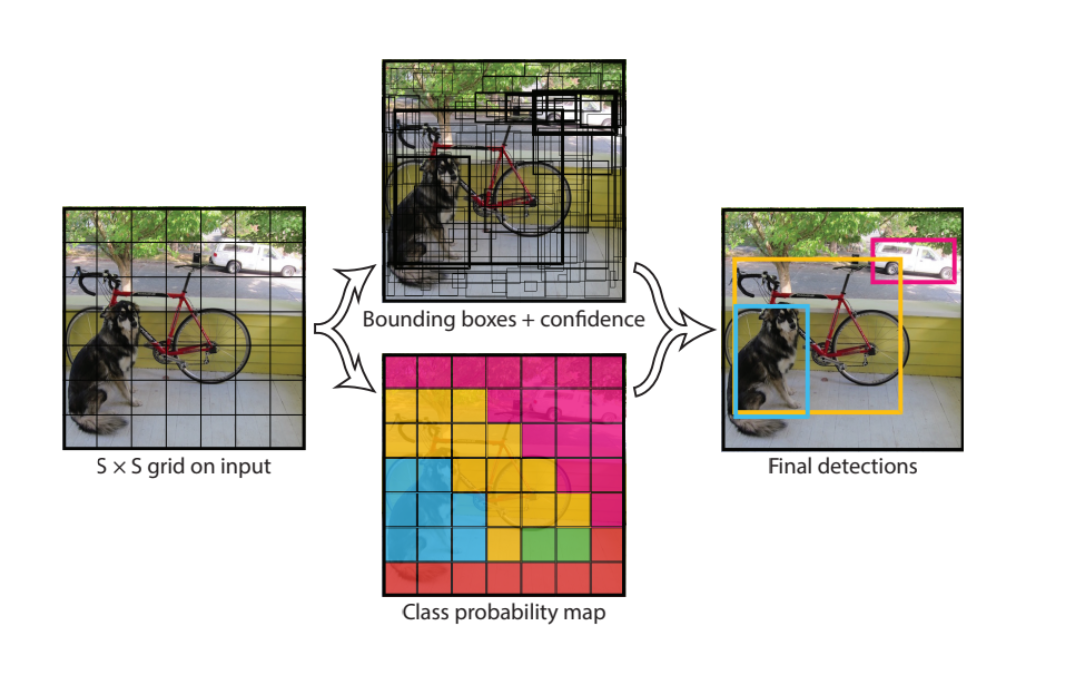
\includegraphics[width=0.45\textwidth]{YOLO.png}
    \caption{YOLO's Working Architecture. Source: [8]}
    \label{fig:external_yolo}
\end{figure}




\subsection{Data Acquisition \& Processing}

i. \textbf{Data Pre-processing} In this part, raw images are resized and normalized to a standard size (e.g., 640 × 640), with pixel values scaled to [0,1] for better training stability. If needed, techniques like flipping, brightness changes, and geometric adjustments are also used to improve model generalization. These steps help ensure better accuracy and adaptability.

ii. \textbf{Model Training} In this part, we will build and improve our training module based on open-source datasets like COCO, Open Images Dataset V7 and ImageNet. By adjusting the model we trained, we aim to improve its accuracy and generalization, making the camera module be better at recognizing road signs for autonomous driving. 

iii. \textbf{Merging i and ii} We will integrate the previous two processes, ensuring that the processed camera-captured images from the first stage achieve training performance comparable to open-source datasets. By aligning preprocessing techniques, normalization, and augmentation strategies with those used in public datasets, we will enhance the model’s learning efficiency. 

\subsection{Hardware Implementation Strategy}

We use common embedded camera modules, such as Raspberry Pi, to deploy and test our training software in real-world conditions. Since deploying algorithms in physical environments often leads to deviations from computer simulations, one of our key objectives is to analyze the causes of these discrepancies and minimize their impact. This helps improve the system’s reliability and ensures smoother performance when transitioning from simulation to real-world application.


\section{Experiment}

Up to now, following the methodology framework, we have completed two main tasks: solution collecting and model testing. We plan to begin with the Model Training section under Data Acquisition and Processing in the methodology. Our initial focus is on identifying existing pre-trained models and evaluating their performance. By testing these models first, we aim to understand their accuracy, efficiency, and suitability for our specific use case.


\subsection{Solution Collecting}

To avoid the unnecessary complexity of building a solution from scratch and to ensure our approach is as scalable as possible, the first step of this project focused on researching existing solutions through multiple information sources. After thorough discussions and evaluations, we finalized three main channels that provided valuable insights and helped shape the direction of our development strategy.

i. \textbf{Open-source Code Platform} Open-source platforms like GitHub offer many smart camera solutions, with ready-to-use code and clear documentation. These resources explain setup, features, and possible uses, making them our top choice for finding existing solutions. They also support collaboration and knowledge sharing, helping us quickly explore scalable options for our project.

ii. \textbf{Capstone Projects in Rice MECE Department} Capstone Projects in Rice MECE Department serve as another crucial research channel. They provide us with the opportunity to engage directly with the teams working on similar initiatives, allowing for valuable discussions and knowledge exchange. Additionally, we can observe and test their hardware and software solutions in real time, gaining first-hand insights into their implementation and performance.

iii. \textbf{Industrial Resources from Rice Faculties} Rice faculty members often have ties to industry, giving access to advanced technologies and real-world smart camera applications. These resources offer insights into best practices and opportunities to collaborate with leading companies. By using these connections, we can learn from proven solutions and apply expert advice to improve our project.

After an initial review of available resources, we selected the GitHub project \textit{Traffic-Light-Detection-Color-Classification} \cite{ExSolution} as the foundation for our work. This project includes three pre-trained YOLOv8 models and utilizes the Ultralytics library to test image datasets with only 17 lines of code. Its simplicity, efficiency, and high potential for extension make it an ideal starting point for further development and customization in our project.


\subsection{Model Testing}

We randomly collected a set of traffic light images from the internet and used the YOLO model from the existing solution \textit{Traffic-Light-Detection-Color-Classification} to perform object detection on these images. The predictions yielded several notable experimental results that highlight the performance and limitations of the model. For detailed information and analysis of these results, please refer to the Results section.

\section{Results}

\subsection{Performance Metrics}
We use the confidence score for performance metrics in our data training process. It measures whether a certain forecast Bounding Box contains the target and its accuracy. Specifically, for each predicted bounding box, YOLO calculates a Confidence Score:

\begin{equation}
  \text{Confidence Score} = \text{P} \times \text{IOU}
\end{equation}
where $\text{P}$ represents the probability of whether the bounding box contains the target, ranging from 0 to 1. IOU(Intersection over Union) indicates the overlap between the predicted bounding Box and the Ground Truth Box, ranging from 0 to 1. Figure shows an example about the COnfidence Score. 


\subsection{Successes \& Challenges}
\vspace{2mm}

i. \textbf{System Efficiency \& Computational Bench-marking:}
As shown in Figure~\ref{fig:successful}, The YOLO-based model successfully detects traffic lights with high precision, proving the validity of the pre-trained model 
\begin{figure}[h]
    \centering
    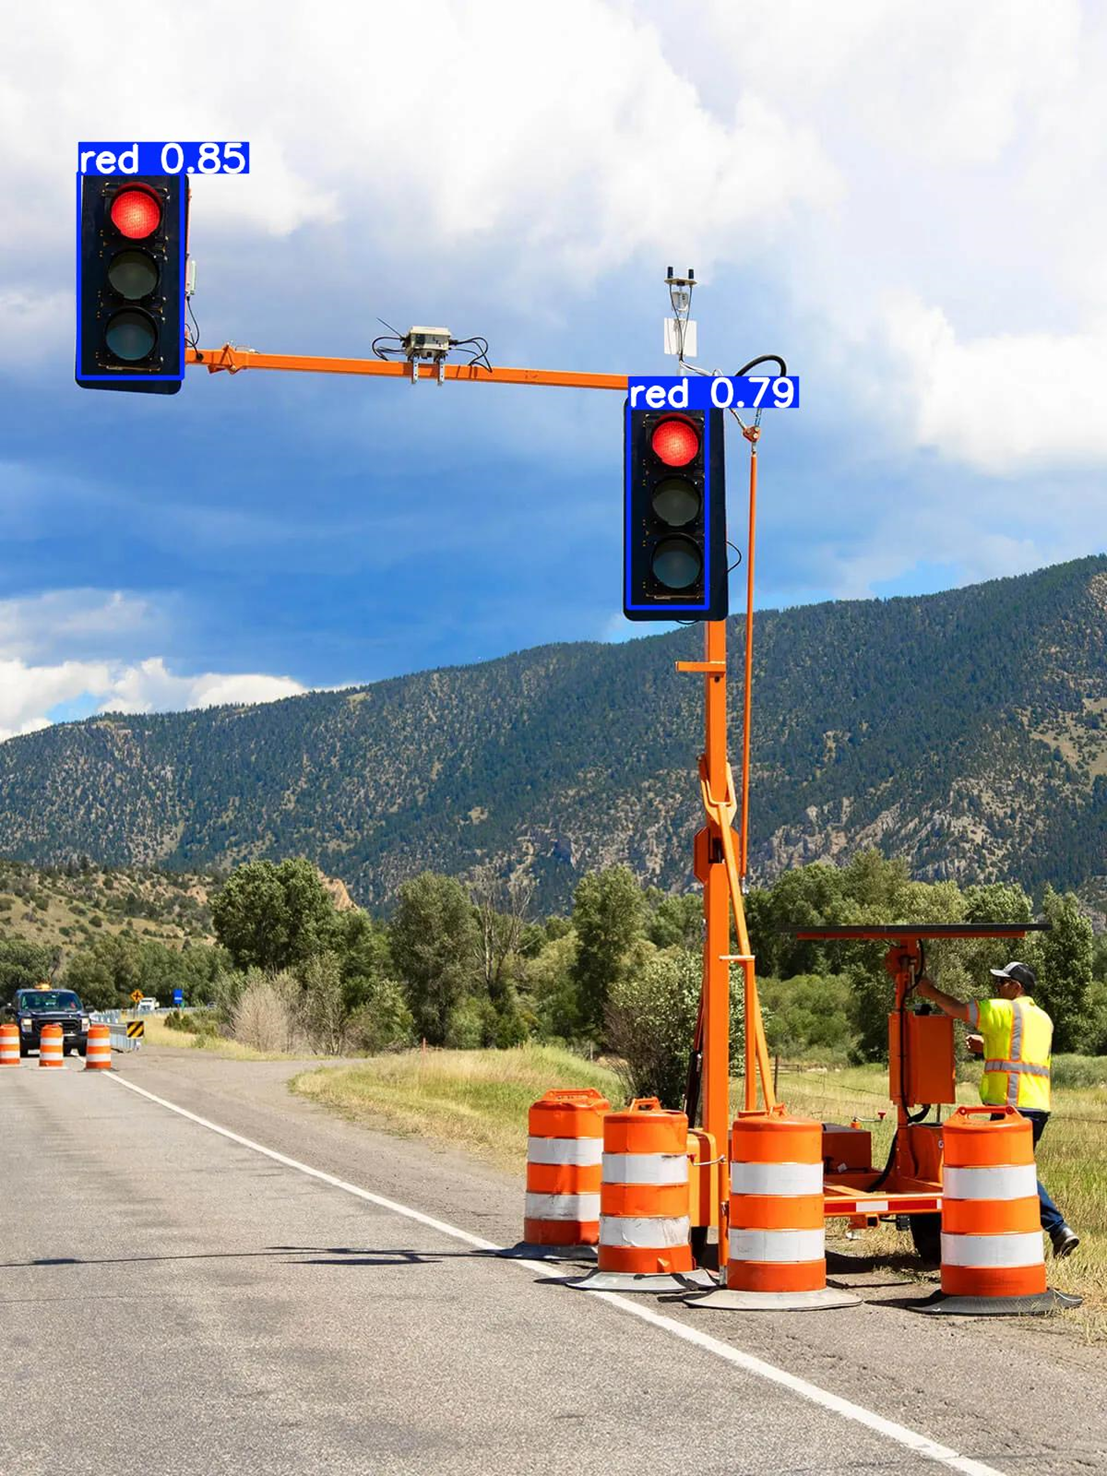
\includegraphics[width=0.3\textwidth]{Result_5.png}
    \caption{Successful Result}
    \label{fig:successful}
\end{figure}



\vspace{1mm}
ii. \textbf{Observed Limitations \& Failure Cases:}
\begin{itemize}
    \item As shown in Figure~\ref{fig:sub1}, the current model is only capable of detecting vertically oriented traffic lights, where the signal bulbs are arranged in a vertical sequence. However, when encountering horizontally oriented traffic lights, the model fails to recognize them effectively. 
    \item As shown in Figure~\ref{fig:sub2}, when traffic lights are too close to the camera, the model fails to detect them accurately. This issue arises due to excessive magnification and loss of contextual information in the frame.
    \item As shown in Figure~\ref{fig:sub3}, the current model can only distinguish the color of traffic lights but cannot determine the direction they indicate. This limitation affects its ability to understand lane-specific signals or arrows within the traffic lights.
\end{itemize}

\begin{figure}[h]
    \centering
    \begin{subfigure}[b]{0.3\textwidth}
        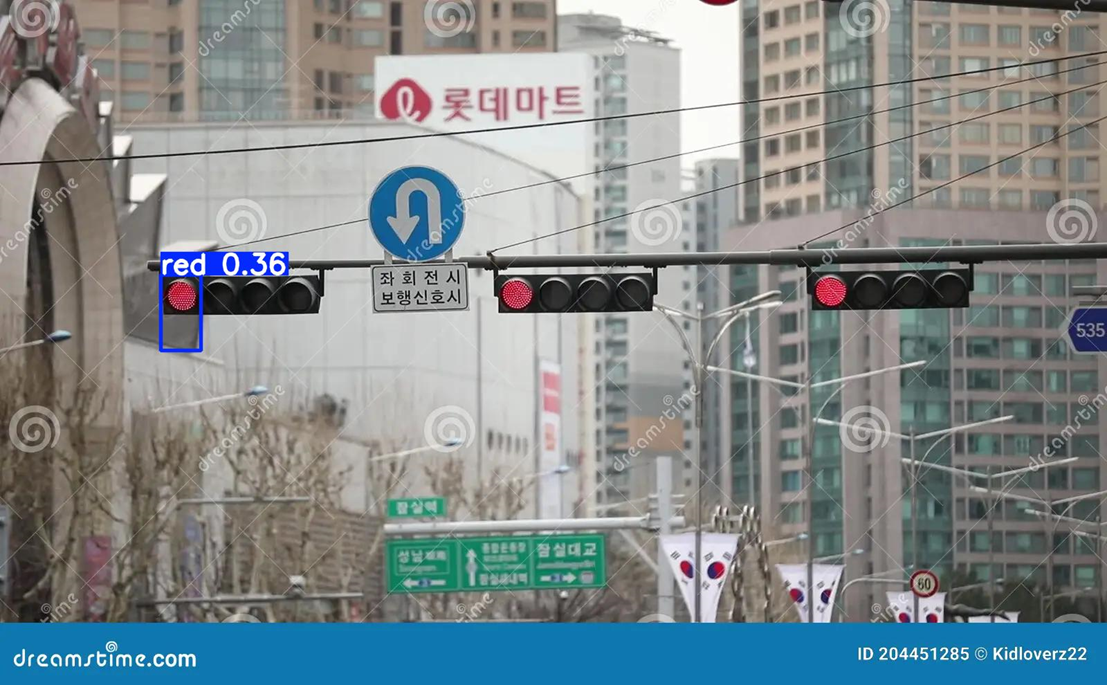
\includegraphics[width=\textwidth]{Result_2.png}
        \caption{The Model do not Work for Horizontal Lights}
        \label{fig:sub1}
    \end{subfigure}
    \hfill
    \begin{subfigure}[b]{0.3\textwidth}
        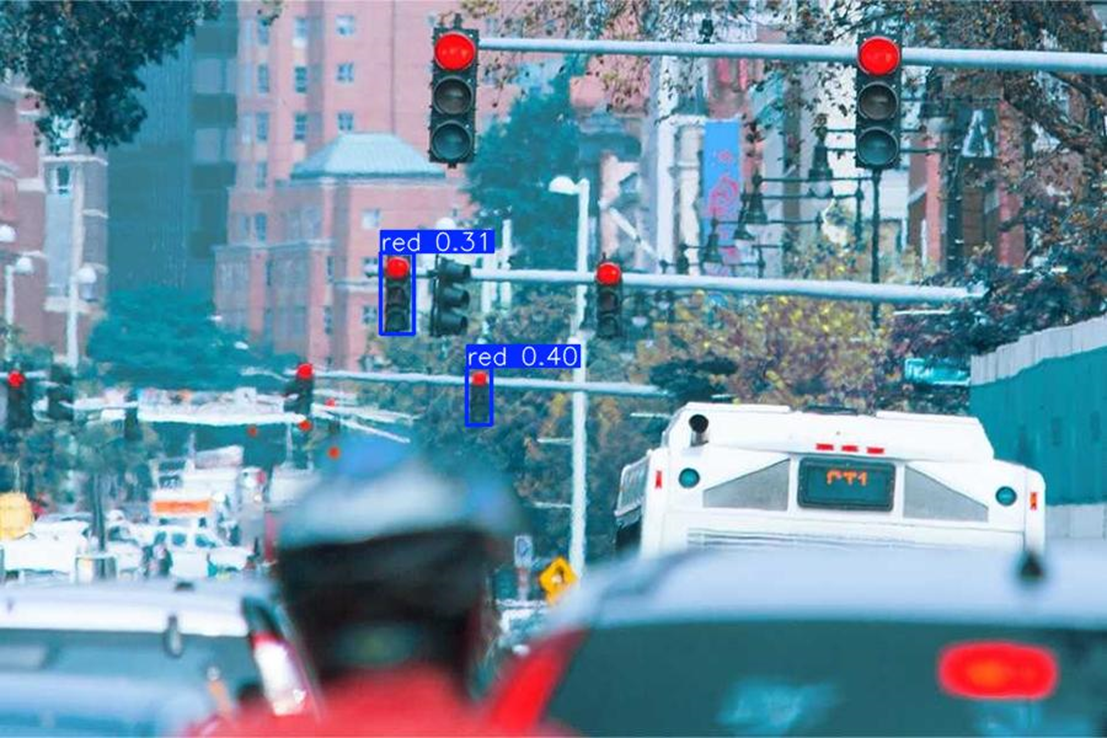
\includegraphics[width=\textwidth]{Result_3.png}
        \caption{The Model do not Work when Traffic Lights are too Close or too Far}
        \label{fig:sub2}
    \end{subfigure}
    \hfill
    \begin{subfigure}[b]{0.3\textwidth}
        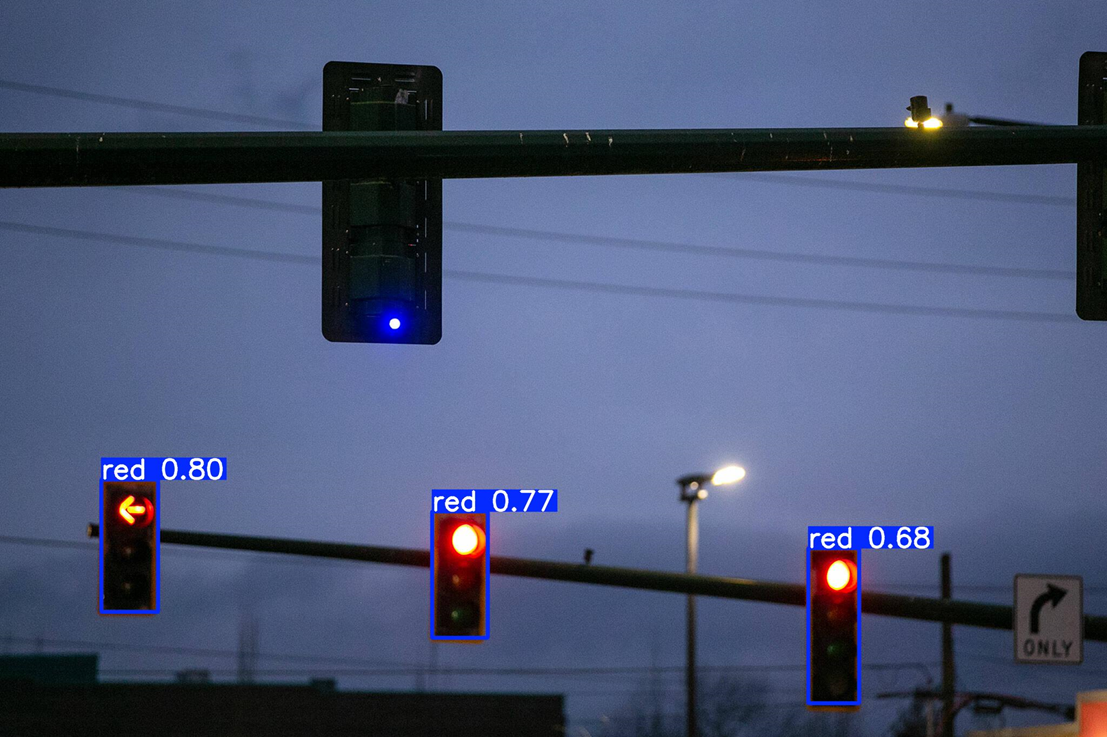
\includegraphics[width=\textwidth]{Result_4.png}
        \caption{The Model cannot Identify Directions
}
        \label{fig:sub3}
    \end{subfigure}
    \caption{Three Representative Failure Results}
    \label{fig:combined}
\end{figure}

\subsection{Compared with FSD}
As shown in Table~\ref{tab:FSD_Feature_Compare}, we compared the model tested in experiment with FSD's feature, giving us a clear direction for our subsequent discussion and future work.

\begin{table*}[t]
\centering
\caption{FSD Main Features}
\label{tab:FSD_Feature_Compare}
\begin{tabular}{|c|>{\centering\arraybackslash}p{9cm}|}  
\hline
\textbf{Feature} & \textbf{Compared with FSD} \\
\hline
Traffic Light Detection & Can only detect colors of vertical lights, being unstable in many situations \\
\hline
Speed Limit Sign Recognition & Unable \\
\hline
Stop Sign and Yield Sign Detection & Unable \\
\hline
Decision Making & Unable \\
\hline
Occlusion Handling & Unable \\
\hline
Nighttime and Low Visibility Performance & Unable \\
\hline
Continuous Learning and Updates & Unable \\
\hline
\end{tabular}
\end{table*}



\section{Discussion}
Combined with the characteristics of YOLO algorithm, we summarized the following three main reasons leading to failure results

i. \textbf{Lack of Diversity in Training Samples} Many existing traffic light datasets predominantly feature vertically oriented traffic lights under standard lighting and distance conditions. Consequently, the model becomes biased toward recognizing only these common configurations. When exposed to less frequent variations, such as horizontally aligned traffic lights or unusual signal designs, the model fails to generalize effectively. This limitation highlights the importance of including a wide range of scenarios in the training data to improve robustness and adaptability to real-world conditions.

ii. \textbf{Mismatch Between Object Size and Image Resolution} For instance, when a traffic light is positioned very close to the camera, it may appear disproportionately large in the image frame, possibly exceeding the receptive field of the model. This can result in incomplete or inaccurate detection due to cropping or distortion. YOLO models rely on anchor boxes tailored to specific object scales, and significant deviations in object size can cause anchor mismatches, reducing detection accuracy. Proper scaling strategies and representation of various object sizes in training data are essential to mitigate this issue.

iii. \textbf{Simplified or Incomplete Labeling in Training Datasets} Traffic light annotations are limited to class labels such as "red light," "green light," or simply "traffic light," without specifying additional attributes like orientation, arrow direction, or light positioning. This lack of detailed annotations prevents the model from learning critical features needed to distinguish subtle differences between similar-looking but functionally different signals. As a result, the model may misclassify or ignore important cues in complex environments. 


\section{Future Work}

In future stages of development, our primary focus will be on enhancing the performance and robustness of our object detection system. It can be divided into 2 parts below:

\subsection{Optimizing the YOLO Model for Traffic Lights}

i. \textbf{Expanding Datasets for YOLO Models:} We aim to expand our dataset by sourcing labeled data that includes various traffic-related visual elements. These will cover directional indicators such as left, straight, and right turns, as well as different types of traffic lights, including pedestrian signals, horizontally aligned lights, and lights viewed from various angles. To complement existing datasets, we will also incorporate manually annotated images to ensure comprehensive coverage and improved model generalization.

ii. \textbf{Configuring the YOLO environment and Training:} we will continue optimizing the YOLO (You Only Look Once) environment and training process, particularly in the detection and recognition of traffic lights. This will involve fine-tuning model parameters, augmenting training data, and implementing strategies to reduce false positives and improve detection under challenging lighting and weather conditions.

iii. \textbf{Adding Decision Making Module:}An essential component of future development will be the integration of a decision-making module. This module will analyze YOLO detection results to determine whether the system should issue a stop or go command based on the state of the traffic light, thereby laying the groundwork for autonomous navigation logic.

\subsection{Training YOLO Models for other objects and Hardware Implementation}

i. \textbf{Training YOLO model for more traffic signs and other objects:}Longer-term goals for this year include extending YOLO model training to cover additional traffic-related objects. These objects include speed limit signs, stop and yield signs, traffic lane markings, and pedestrians. Once trained, these models will be tested and optimized using real-time images and video streams to evaluate performance in dynamic environments.

ii. \textbf{Hardware Implementation and further optimizing:}Finally, we plan to implement our models in hardware platforms to validate real-world applicability. This step will involve transferring the trained models to embedded systems or edge devices, where further optimization for latency, power efficiency, and reliability will be performed. These efforts will help bring the system closer to deployment in practical autonomous driving or smart traffic management applications.





% if have a single appendix:
%\appendix[Proof of the Zonklar Equations]
% or
%\appendix  % for no appendix heading
% do not use \section anymore after \appendix, only \section*
% is possibly needed

% use appendices with more than one appendix
% then use \section to start each appendix
% you must declare a \section before using any
% \subsection or using \label (\appendices by itself
% starts a section numbered zero.)
%


%\appendices
%\section{}


% use section* for acknowledgment
\section*{Acknowledgment}


The authors would like to thank to the KTMtechnology for sponsoring this Smart Camera project for MECE ELEC 594 program.


% Can use something like this to put references on a page
% by themselves when using endfloat and the captionsoff option.
\ifCLASSOPTIONcaptionsoff
  \newpage
\fi



% trigger a \newpage just before the given reference
% number - used to balance the columns on the last page
% adjust value as needed - may need to be readjusted if
% the document is modified later
%\IEEEtriggeratref{8}
% The "triggered" command can be changed if desired:
%\IEEEtriggercmd{\enlargethispage{-5in}}

% references section

% can use a bibliography generated by BibTeX as a .bbl file
% BibTeX documentation can be easily obtained at:
% http://mirror.ctan.org/biblio/bibtex/contrib/doc/
% The IEEEtran BibTeX style support page is at:
% http://www.michaelshell.org/tex/ieeetran/bibtex/
%\bibliographystyle{IEEEtran}
% argument is your BibTeX string definitions and bibliography database(s)
%\bibliography{IEEEabrv,../bib/paper}
%
% <OR> manually copy in the resultant .bbl file
% set second argument of \begin to the number of references
% (used to reserve space for the reference number labels box)
\begin{thebibliography}{1}

\bibitem{SelfDriving}
S. Santosh Kumar, \emph{Self-Driving Car Using Neural Networks and
Computer Vision}\hskip 1em plus
  0.5em minus 0.4em\relax IEEE ,IIHC, 2022.


\bibitem{Controlling Mobile Robot}
Khansaa Dheyaa Ismael, \emph{Controlling Mobile Robot Navigation Equipped with Computer Vision Perception for Text using OCR
Technique}\hskip 1em plus
 0.5em minus 0.4em\relax IEEE, SSD, 2024.

 \bibitem{Smart Cameras}
David Brady, \emph{Smart Cameras}\hskip 1em plus
 0.5em minus 0.4em\relax  Duke university, 2020.

\bibitem{Design and Realization}
Xuanxuan Hong, \emph{Design and Realization of Fire Detection Using
Computer Vision Technology}\hskip 1em plus
 0.5em minus 0.4em\relax  IEEE, CCDC, 2019

\bibitem{Camera-trap-classifier}
Macro-willi, \emph{Camera-trap-classifier}\hskip 1em plus
 0.5em minus 0.4em\relax  GitHub repository, 2019.
[Online]

\bibitem{UniScene}
Chaytonmin, \emph{UniScene}\hskip 1em plus
 0.5em minus 0.4em\relax  GitHub repository, 2023.
[Online]

\bibitem{Autodrone}
MECE students, \emph{Autodrone}\hskip 1em plus
 0.5em minus 0.4em\relax  Rice Unv. ,GitHub repository, 2024.
[Online]

\bibitem{fasterrcnn}
S.~Ren, K.~He, R.~Girshick, and J.~Sun, \emph{Faster R-CNN: Towards Real-Time Object Detection with Region Proposal Networks}\hskip 1em plus 0.5em minus 0.4em\relax arXiv preprint arXiv:1506.02640, 2015. [Online]. Available: \url{https://arxiv.org/abs/1506.02640}

\bibitem{FSD}
Tesla, \emph{Autopilot and Full Self-Driving (Supervised)}\hskip 1em plus 0.5em minus 0.4em\relax Tesla

\bibitem{Autopilot}
K. Nived Maanyu, \emph{A Study on Tesla Autopilot}\hskip 1em plus 0.5em minus 0.4em\relax Sreenidhi Institute of Science And Technology, 2020 

\bibitem{ExSolution}
Syazvinski, \emph{Traffic-Light-Detection-Color-Classification}\hskip 1em plus
 0.5em minus 0.4em\relax GitHub repository, 2023.
[Online]

\bibitem[Fig.4]
*Carousel, \emph{Manderfield Highway Information}\hskip 1em plus 0.5em minus 0.4em\relax Beaver County, 2024

\bibitem[Fig.5-(a)]
*Kidloverz22, \emph{Seoul,South Korea-March 2019: Close up image of traffic light changes color with Korean traffic street sign}\hskip 1em plus 0.5em minus 0.4em\relax Dreamstime.com

\bibitem[Fig.5-(b)]
*Katherine Tweed, \emph{Better Traffic Light Simulations Could Cut Travel Time and Gas Use}c IEEE Spectrum, 2014
\bibitem[Fig.5-(c)]
*Ben Watanabe, \emph{Those blue lights on traffic signals help nab red-light runners}\hskip 1em plus 0.5em minus 0.4em\relax HeraldNet, 2022

\end{thebibliography}



% biography section
% 
% If you have an EPS/PDF photo (graphicx package needed) extra braces are
% needed around the contents of the optional argument to biography to prevent
% the LaTeX parser from getting confused when it sees the complicated
% \includegraphics command within an optional argument. (You could create
% your own custom macro containing the \includegraphics command to make things
% simpler here.)
%\begin{IEEEbiography}[{\includegraphics[width=1in,height=1.25in,clip,keepaspectratio]{mshell}}]{Michael Shell}
% or if you just want to reserve a space for a photo:


% insert where needed to balance the two columns on the last page with
% biographies
%\newpage


% You can push biographies down or up by placing
% a \vfill before or after them. The appropriate
% use of \vfill depends on what kind of text is
% on the last page and whether or not the columns
% are being equalized.

%\vfill

% Can be used to pull up biographies so that the bottom of the last one
% is flush with the other column.
%\enlargethispage{-5in}



% that's all folks
\end{document}


